\scanpage{13}
\mspage{10}
Now if $i\leq n$, we shall have
\[
\left\{\quad\Lambda\pi_{i0}=0,\qquad\Lambda\pi_{i\alpha}=L^{\alpha-1}w_{i-2\alpha}L^{n-i+\alpha}\pi_{i\alpha}\quad\text{if }\alpha\geq1,\right.
\tag{6.12}
\]
\deleted{and if $j>n$, we shall have
\[
\Lambda\pi_{j\alpha}=L
\tag{6.12}
\]}
\[
\Lambda\pi_{2n-i,\alpha}=L^{n-i+\alpha-1}w_{i-2\alpha}\deleted{\unsure{\pi_{2n-i,\alpha}}}L^\alpha\pi_{2n-i,\alpha}\quad(\text{if }i\leq n-1)
\tag{6.13}
\]
\margin{The conditions under consideration obviously imply (iv) : prove that (iv) implies (ii). It suffices in fact to prove that we then have $\pi_i=\pi'_i$. \uline{Proof to be supplied.}}

\uline{Remark} Here is a system of conditions uniquely determining the elements $\Lambda\in\mathcal E^{(2)},\ \pi_{i,\alpha}\in\mathcal E^{(0)}$ in terms of $L$, and of the $\pi_i\deleted{\unsure{\alpha}}$ (for which we already have an intrinsic characterization elsewhere, in terms of the graded ring $\mathcal E$) :
\margin{\deleted{$\unsure{\pi_{2n-i}}$}}
\[
\left\{\begin{aligned}
\textcircled{1}\quad &(\Lambda^{n-i}L^{n-i}-1)\pi_i=0
\qquad\textcircled{2}\quad\deleted{\pi_{2n-i}}(L^{n-i}\Lambda^{n-i}-1)\deleted{\pi_{2n-i}}\pi_{2n-i}=0\\
\textcircled{3}\quad &\pi_{i,\alpha}=L^\alpha\deleted{\unsure{w_{i-2\alpha}}}\inserted{\Lambda^{n-i+2\alpha}}L^{n-i+\alpha}\bigl(1-\sum_{\alpha'>\alpha}\pi_{i,\alpha'}\bigr)\\
\textcircled{4}\quad &\pi_{2n-i,\alpha}=L^{n-i}\pi_{i,\alpha}\Lambda^{n-i}\\
&\deleted{\Lambda=\sum_{j,\alpha}\Lambda\pi_{j\alpha}}\\
\textcircled{5}\quad &\Lambda\pi_{i,0}=0\qquad\deleted{\unsure{\alpha}}\\
\textcircled{6}\quad &\Lambda\pi_{i\alpha}=L^{\alpha-1}\Lambda^{n-i+2\alpha}L^{n-i+\alpha}\pi_{i\alpha}\quad\text{if }\alpha\geq1\\
\textcircled{7}\quad &\Lambda\pi_{2n-i,\alpha}=L^{n-i+\alpha-1}\Lambda^{n-i+2\alpha}L^\alpha\pi_{2n-i,\alpha}\quad\text{if }\alpha\leq n-1\\
\textcircled{8}\quad &\Lambda=\sum_{j,\alpha}\Lambda\pi_{j\alpha}
\end{aligned}\right.
\tag{6.14}
\]
(in all these formulas, we assume $i\leq n$).

In these eight formulas, one can moreover replace the last four by the following \inserted{\figure{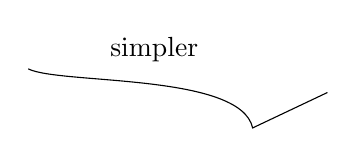
\begin{tikzpicture}[x=1cm,y=1cm]
\node at (0,.35) {simpler};
\draw (-1.6,.1) .. controls (-1.2,-.1) and (1.1,.05) .. (1.25,-.65) -- (2.2,-.2);
\end{tikzpicture}}} ones :
\mspage{12}
